
\section{Overview}\label{sect:Overview}

This tutorial is intended to provide a introduction to the basics of Markov chain Monte Caro (MCMC) using the  Metropolis-Hastings algorithm. This will provide a brief introduction to MCMC moves as well as prior distributions. We begin with a simple example of estimating the probability distribution of an archer's ability to shoot at a target, and the distance those arrows land from the center. We will simulate data using this example and attempt to estimate the posterior distribution using a variety of MCMC moves. 

\section{Modeling an archer's shots on a target}\label{sect:Exercise}

We'll begin our exploration of Bayesian inference with a simple archery model.
In this model, we imagine shooting $n$ arrows at a target and measuring the distance distance of each arrow from the target's center.
Let's assume that the distance of each arrow from the bullseye follows an exponential distribution.
Further, we assume the archer has an inherent ability to shoot arrows at an average average distance $\mu$.
Then, the probability density of each arrow distance $x_i$ is
\begin{align*}
P(x_i \mid \mu) = \frac{1}{\mu} e^{-x_i/\mu}
\end{align*}
Simple intuition suggests that, given that we observe $n$ arrows, the maximum-likelihood estimate (MLE) of $\mu$ is simply the average of all the arrow distances $\bar x = \frac{1}{n}\sum_{i=1}^n x_i$.
This is indeed the maximum likelihood estimate!
In fact, given $n$ arrows whose distances follow an exponential distribution, it turns out that the observed average $\bar x$ follows a gamma distribution, with parameters $n$ and $n/\mu$.
\begin{align*}
P(\bar x \mid \mu,n) = \frac{(n/\mu)^n}{\Gamma(n)} {\bar x}^{n-1}e^{-n\bar x /\mu}
\end{align*}
In this case, the average $\bar x$ acts as a \emph{sufficient statistic} for $\mu$. This means that it tells us everything we need to know about $\mu$.
Therefore, we will use a Gamma$(n, n\mu)$ distribution on $\bar x$ as the likelihood of our data.

From Bayes' theorem, the \emph{posterior distribution} of $\mu$ given $\bar x$, $P(\mu \mid \bar x)$, is:
\begin{align*}
\overbrace{P(\mu \mid \bar x)}^{\text{posterior distribution}} = \frac{ \overbrace{P(\bar x \mid \mu)}^{\text{likelihood}} \times \overbrace{P(\mu)}^{\text{prior}}}{\underbrace{P(\bar x)}_{\text{marginal likelihood}}}
\end{align*}
The take-home message here is that, if we're interested in doing Bayesian inference for the archery model, we need to specify a \emph{likelihood function} and a \emph{prior distribution} for $\mu$.
In virtually all practical cases, we cannot compute the posterior distribution directly and instead use numerical procedures, such as a Markov chain Monte Carlo (MCMC) algorithm.
Therefore, we will also have to write an MCMC algorithm that samples parameter values in the frequency of their posterior probability.

We'll use a simple exponential distribution as a prior on the parameter of the model, $\mu$.
The exponential distribution has one parameter $\alpha$ representing our prior belief about the mean arrow distance (Figure~\ref{fig:exponential_distribution}).
Different choices for $\alpha$ represent different prior beliefs.
\begin{figure}[h!]
\centering
\fbox{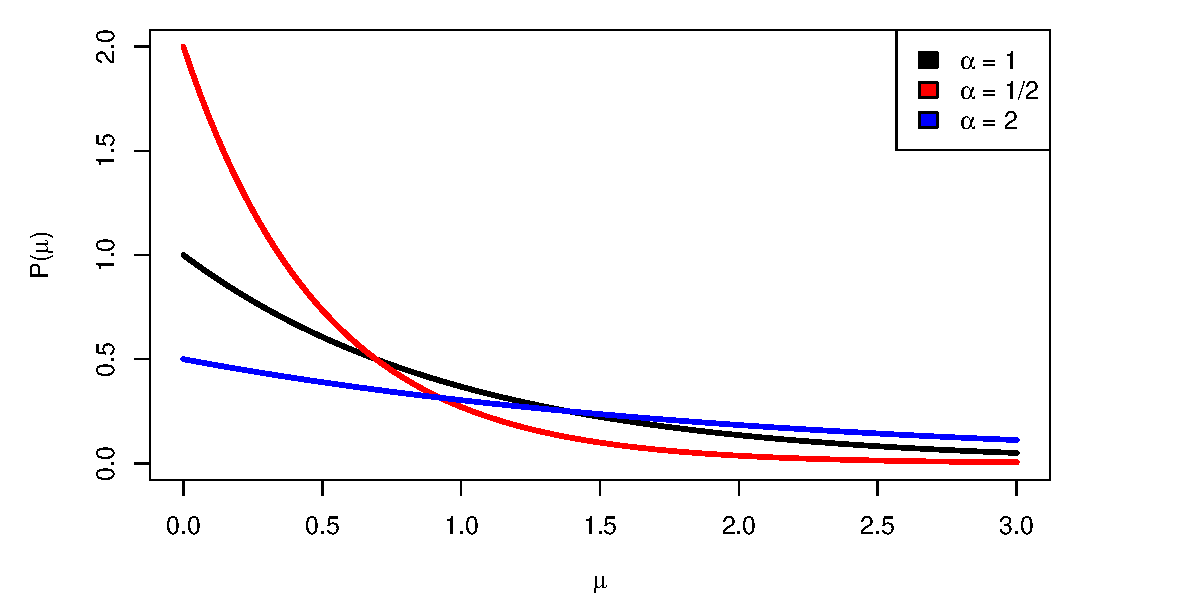
\includegraphics[width=0.7\linewidth,angle=0]{\ResourcePath figures/exp.pdf}}
\label{fig:exponential_distribution}
\caption{An exponential distribution with one parameter $\alpha$. This distribution is used as a prior distribution on the average arrow distance  $\mu$.
Here we show different curves for the exponential distribution when using different parameters.}
\end{figure}

Figure~\ref{fig:archery_model} shows the graphical model for the archery model.
This nicely visualizes the dependency structure in the model.
We see that the parameter $\alpha$ is drawn in a solid square, representing that this variable is constant.
From this variables, we see an arrow going into the variable $\mu$.
That simply means that $\mu$ depends on $\alpha$.
More specifically, $\mu$ is a stochastic variable (shown as a solid circle) and drawn from an exponential distribution with parameter $\alpha$.
Then, we have another constant variable, $n$.
Finally, we have the observed data $\bar x$ which is drawn from a gamma distribution with parameters $\mu$ and $n$, as can be seen by the arrows going into $x$.
Furthermore, the solid circle of $\bar x$ is shaded which means that the variable has data attached to it.
\begin{figure}[h!]
\centering
\fbox{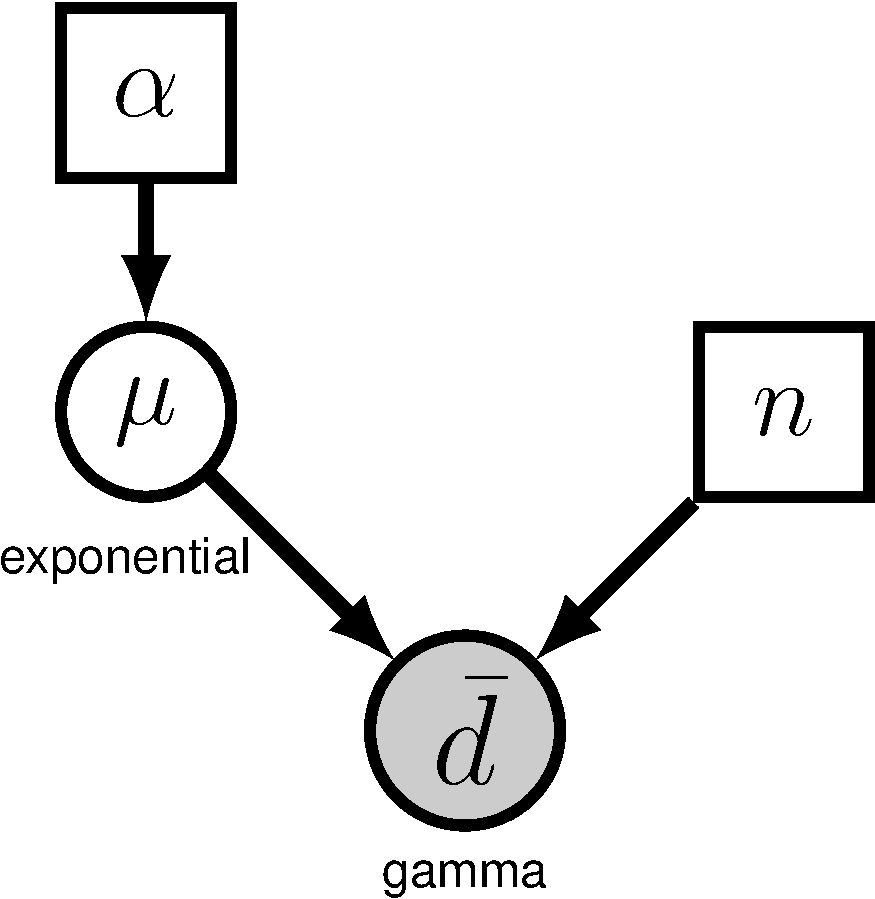
\includegraphics[width=1.8in,angle=0]{\ResourcePath figures/archery_graphical_model.pdf}}
\label{fig:archery_model}
\caption{A graphical model for the archery model.}
\end{figure}

\section{Writing an MCMC from Scratch}

\impmark Make yourself familiar with the example script called \emph{archery\_MH.Rev} which shows the code for the following sections. Then, start a new and empty script and follow each step provided in the \colorbox{shadecolor}{blue boxes}.

\subsection{The Metropolis-Hastings Algorithm}
Though \RevBayes implements efficient and easy-to-use Markov chain Monte Carlo algorithms, we'll begin by writing one ourselves to gain a better understanding of the moving parts.
The Metropolis-Hastings MCMC algorithm \citep{Metropolis1953,Hastings1970} proceeds as follows:

\begin{enumerate}
	\item Generate initial values for the parameters of the model (in this case, $mu$).
	\item Propose a new value (which we'll call $mu^\prime$) for some parameters of the model, (possibly) based on their current values 
	\item Calculate the acceptance probability, $R$, according to:
	\begin{align*}
		R = \text{min}\left\{1, \frac{P(\bar x \mid \mu^\prime)}{P(\bar x \mid \mu)} \times \frac{P(\mu^\prime)}{P(\mu)} \times \frac{q(\mu)}{q(\mu^\prime)} \right\}
	\end{align*}
	\item Generate a uniform random number between 1 and 0. If it is less than $R$, accept the move (set $\mu = \mu^\prime$). Otherwise, keep the current value of $\mu$.
	\item Record the values of the parameters.
	\item Return to step 2 many many times, keeping track of the value of $\mu$.
\end{enumerate}

\subsection{Reading in the data}
Actually, in this case, we're just going to simulate some data on the spot.
Feel free to alter these values to see how they influence the posterior distribution
{\tt \begin{snugshade*}
\begin{lstlisting}    
# Simulate some data (i.e. shoot some arrows)
# First we need the number of arrows to shoot
n = 10
# Then we need some true mean distance
mu_true = 1
# Simulate the observed mean distance of the arrows we shot
arrow_mean = rgamma(1, n, n/mu_true)[1]
\end{lstlisting}
\end{snugshade*}}

\subsection{Initializing the Markov chain}
We have to start the MCMC off with some initial parameter values.
One way to do this is to randomly draw values of the parameters (just $\mu$, in this case) from the prior distribution.
We'll assume a simple exponential prior distribution; that is, one with $\alpha = 1$.
{\tt \begin{snugshade*}
\begin{lstlisting}
# Initialize the chain with some starting value
alpha = 1.0
mu = rexp(1, alpha)[1]
\end{lstlisting}
\end{snugshade*}}

\subsubsection{Likelihood function}
We also need to specify the likelihood function.
We use the gamma distribution for the likelihood. Since the likelihood is defined only for values of $\mu$ greater than 0, we return a likelihood of 0.0 if $\mu$ is negative:
{\tt \begin{snugshade*}
\begin{lstlisting}
# Define the likelihood function on the mean 
function likelihood(mu){
    if(mu < 0.0)
        return 0.0

    return dgamma(arrow_mean, n, n/mu, log=false)
}
\end{lstlisting}
\end{snugshade*}}

\subsubsection{Prior distribution}
Similarly, we need to specify a function for the prior distribution.
Here, we use the exponential probability distribution for the prior on $\mu$:
{\tt \begin{snugshade*}
\begin{lstlisting}    
# Define the prior function on the mean 
function prior(mu){
    if(mu < 0.0)
        return 0.0

    return dexp(mu, alpha, log=false)
}
\end{lstlisting}
\end{snugshade*}}


\subsubsection{Monitoring parameter values}
Additionally, we are going to monitor, \IE store, parameter values into a file during the MCMC simulation.
For this file we need to write the column headers:
{\tt \begin{snugshade*}
\begin{lstlisting}
# Prepare a file to log our samples
write("iteration","mu","\n",file="archery_MH.log")
write(0,mu,"\n",file="archery_MH.log",append=TRUE)
\end{lstlisting}
\end{snugshade*}}
(You may have to change the newline characters to \texttt{"$\backslash$r$\backslash$n"} if you're using a Windows operating system.)
We'll also monitor the parameter values to the screen, so let's print the initial values:
{\tt \begin{snugshade*}
\begin{lstlisting}
# Print the initial values to the screen
print("iteration","mu")
print(0,mu)
\end{lstlisting}
\end{snugshade*}}

\subsection{Writing the MH Algorithm}
At long last, we can write our MCMC algorithm.
First, we define how often we print to file (\IE monitor), which is also often called thinning.
If we set the variable \cl{printgen} to 1, then we will store the parameter values every iteration; if we choose \cl{printgen=10} instead, then only every $10$th iteration.
{\tt \begin{snugshade*}
\begin{lstlisting}    
printgen = 10
\end{lstlisting}
\end{snugshade*}}
We will repeat this resampling procedure many times and iterate the MCMC using a \texttt{for} loop:
{\tt \begin{snugshade*}
\begin{lstlisting}    
# Write the MH algorithm
reps = 10000 
for(rep in 1:reps){
\end{lstlisting}
\end{snugshade*}}
(remember to close your \texttt{for} loop at the end).

The first thing we do in the first generation is generate a new value of $\mu^\prime$ to evaluate.
We'll simply propose a new value of $\mu$ from a the prior distribution.
Note that in this first example we do not condition new parameter values on the current value.
{\tt \begin{snugshade*}
\begin{lstlisting}    
    # Propose a new value of p
    mu_prime <- rexp(n=1, alpha)[1]
\end{lstlisting}
\end{snugshade*}}

Next, we compute the proposed likelihood and prior probabilities, as well as the acceptance probability, $R$:
{\tt \begin{snugshade*}
\begin{lstlisting}    
    # Compute the acceptance probability
    R = ( likelihood(mu_prime)/likelihood(mu) ) * ( prior(mu_prime)/prior(mu) )
\end{lstlisting}
\end{snugshade*}}

Then, we accept the proposal with probability $R$ and reject otherwise:
{\tt \begin{snugshade*}
\begin{lstlisting}    
    # Accept or reject the proposal
    u <- runif(1,0,1)[1]
    if(u < R){
        # Accept the proposal
        mu <- mu_prime
    }
\end{lstlisting}
\end{snugshade*}}

Finally, we store the current value of $\mu$ in our log file.
Here, we actually check if we want to store the value during this iteration.
{\tt \begin{snugshade*}
\begin{lstlisting}
    if ( (rep % printgen) == 0 ) {
        # Write the samples to a file
        write(rep,mu,"\n",file="archery_MH.log",append=TRUE)
        # Print the samples to the screen
        print(rep,mu)
    }
} # end MCMC\end{lstlisting}
\end{snugshade*}}


\subsection{Exercise 1}

\begin{enumerate}[label=\textnormal{Step \arabic*)}]
	\item Write and execute this script (there is also an example file called \emph{archery\_MH.Rev}).
	\item The \texttt{.log} file will contain samples from the posterior distribution of the model! Open the file in \Tracer to learn about various features of the posterior distribution, for example: the posterior mean or the 95\% credible interval.
\end{enumerate}
Pretty awesome, right?

Below we show an example of the obtained output in \Tracer.
Specifically, Figure~\ref{fig:mcmc_samples} shows the sample trace (left) and the estimated posterior distribution of $\mu$ (right).
There are other parameters, such as the posterior mean and the 95\% HPD (highest posterior density) interval, that you can obtain from \Tracer.
\begin{figure}[h!]
\centering
\fbox{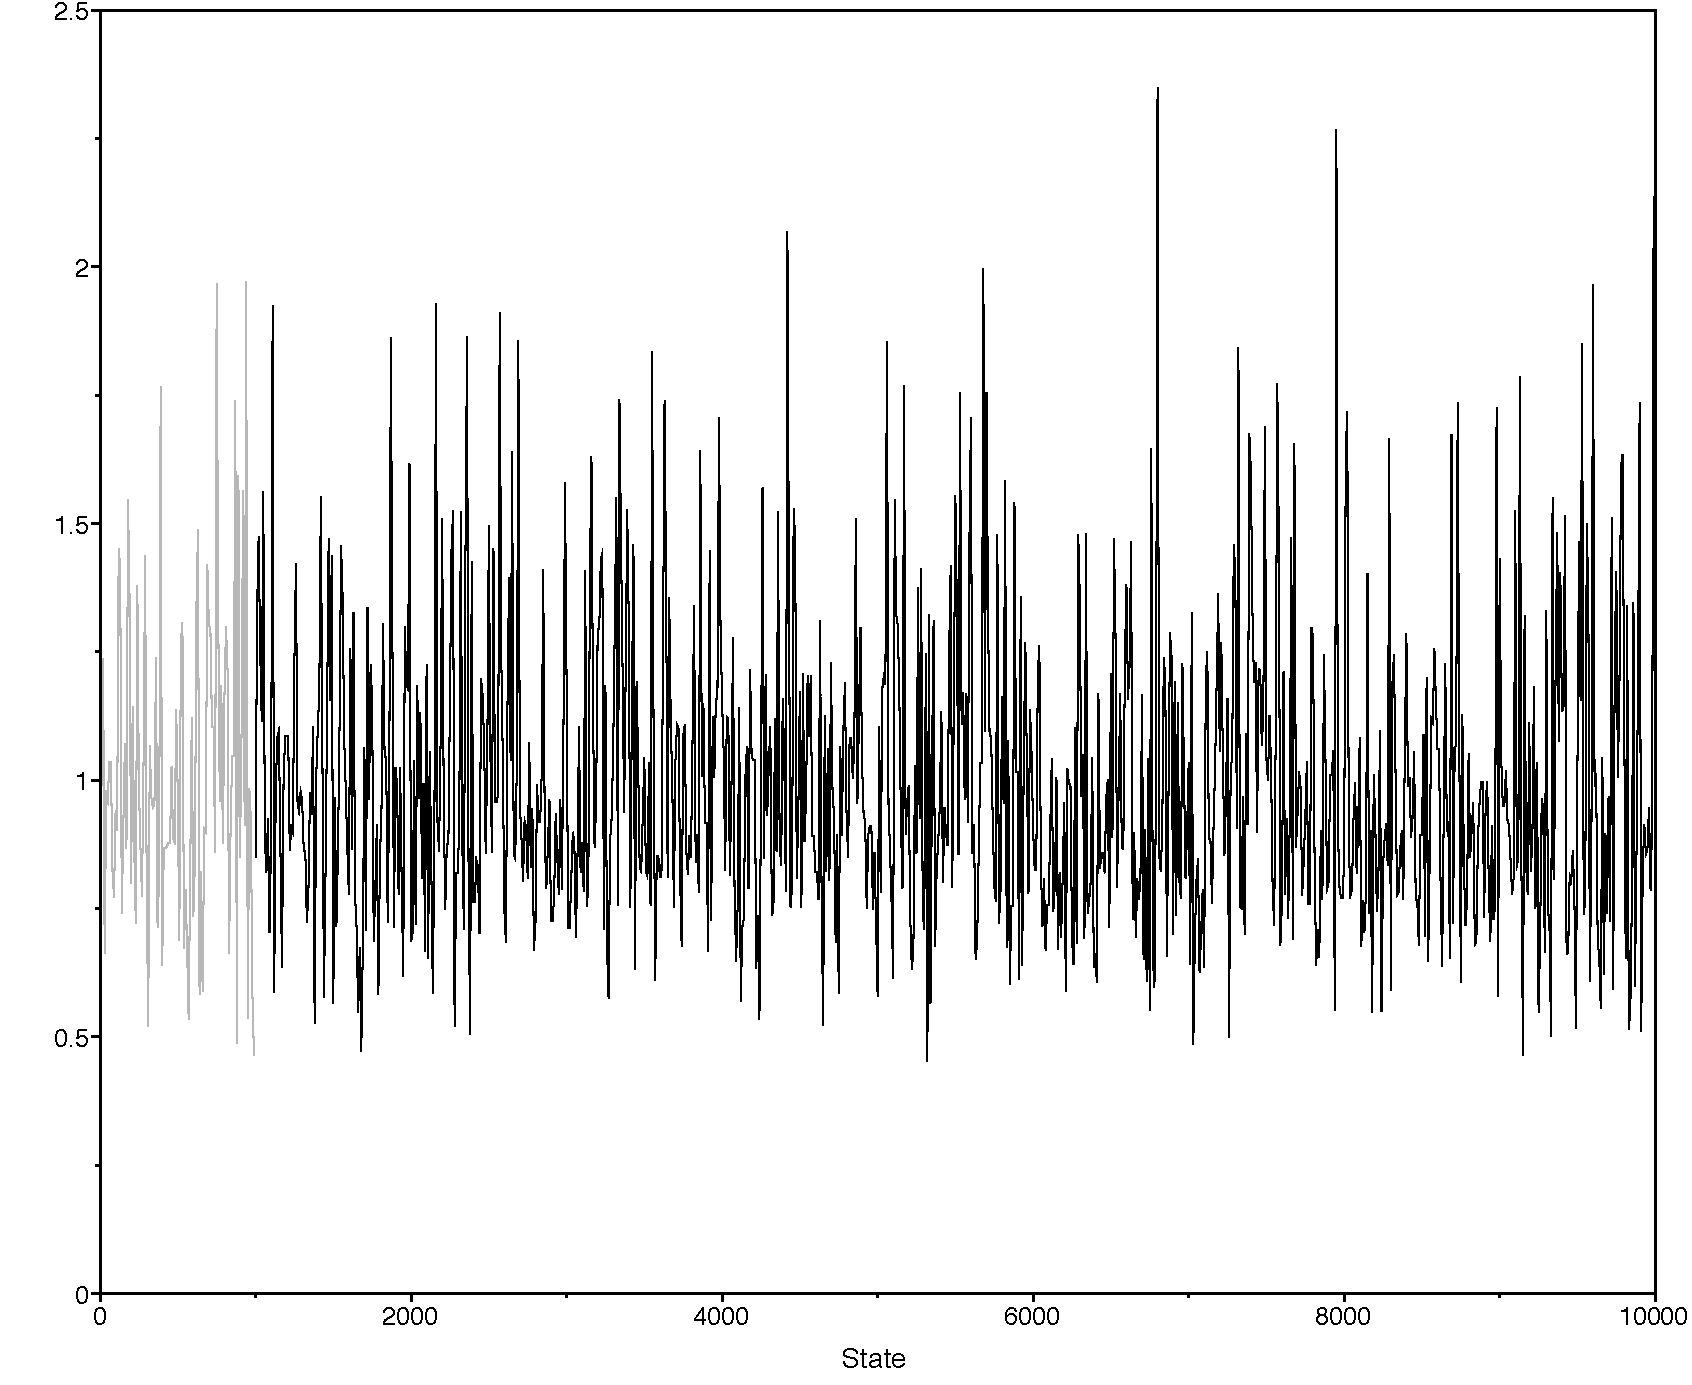
\includegraphics[width=0.45\linewidth,angle=0]{\ResourcePath figures/archery_MCMC_Trace.pdf}
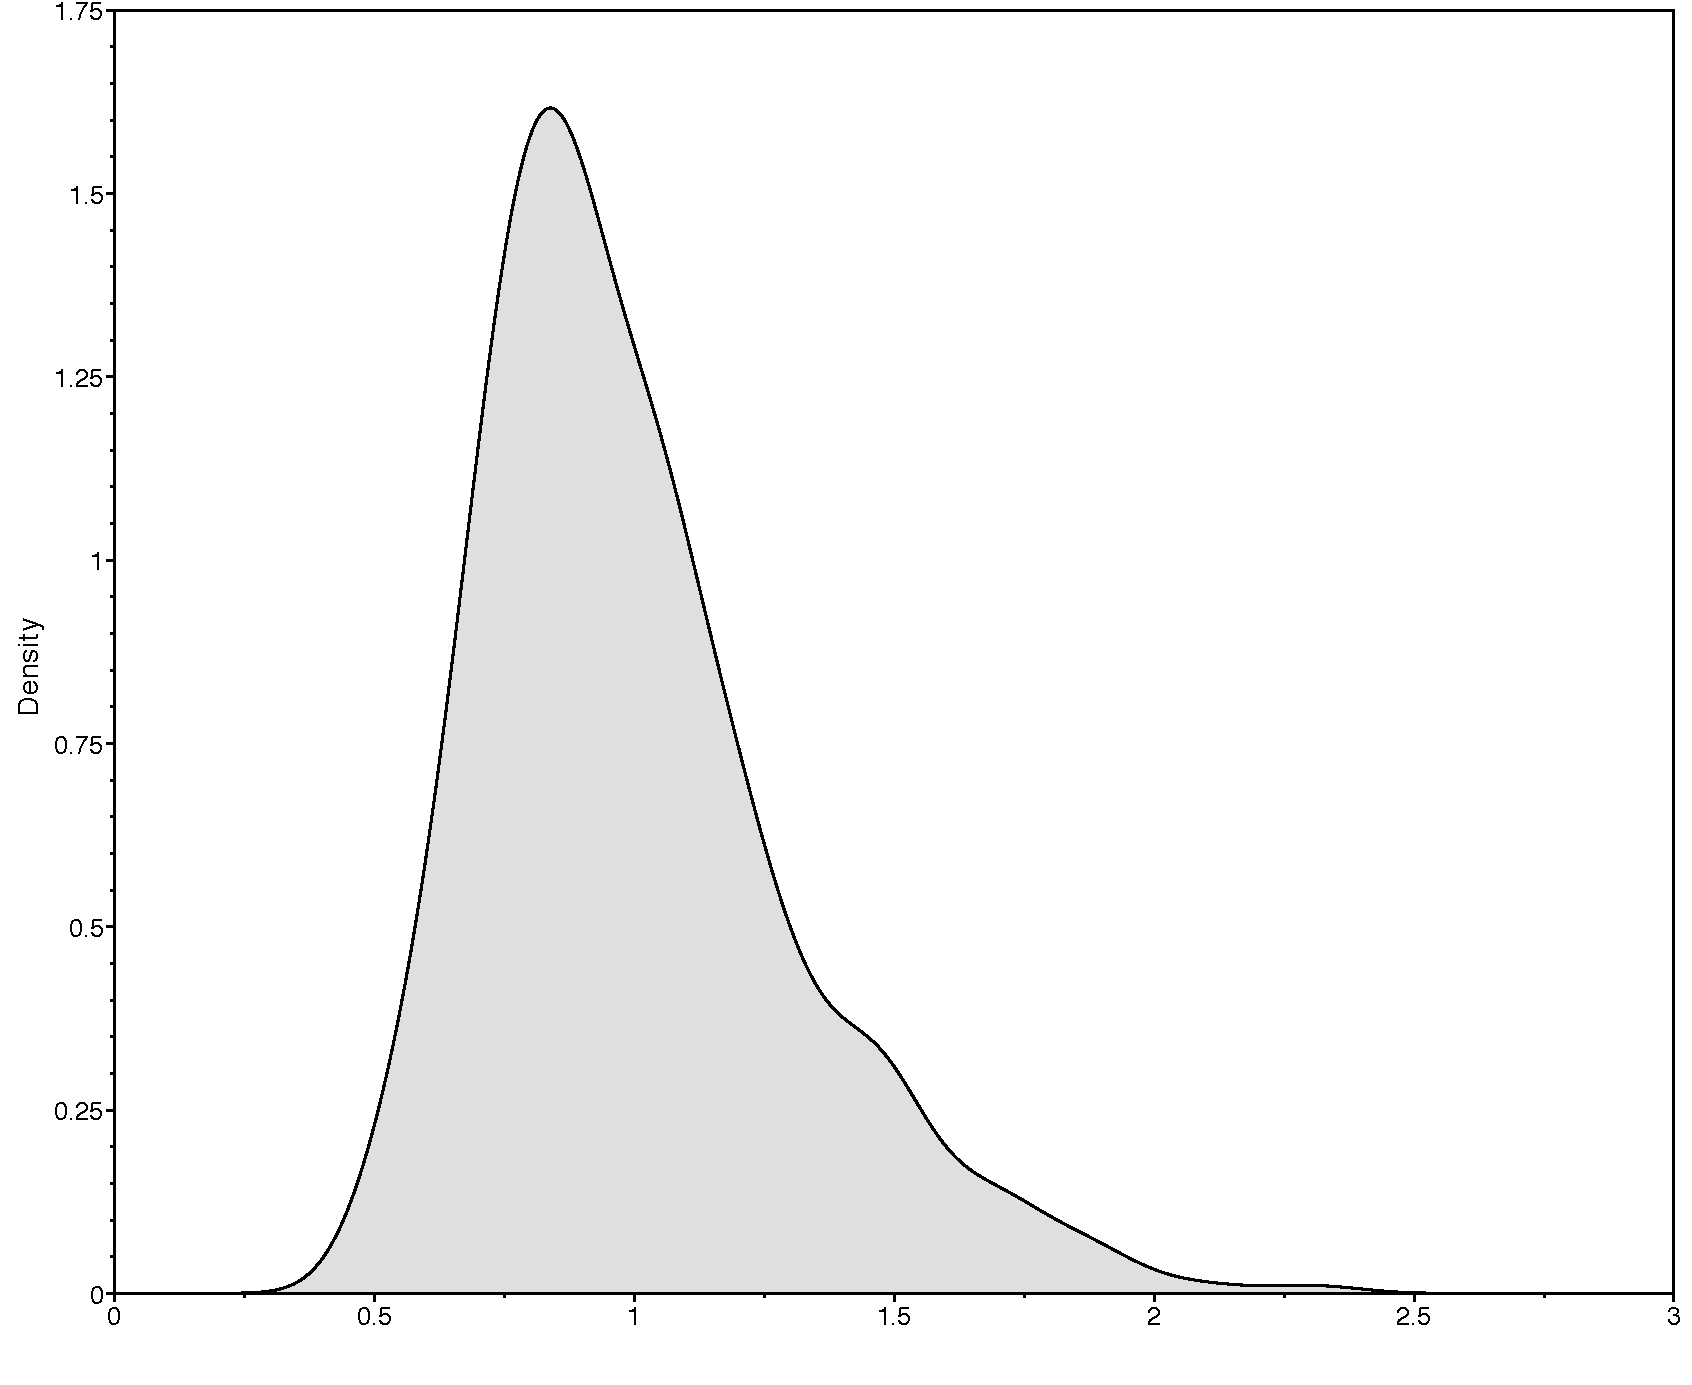
\includegraphics[width=0.45\linewidth,angle=0]{\ResourcePath figures/archery_MCMC_distribution.pdf}}
\label{fig:mcmc_samples}
\caption{Left: The \emph{Trace} of sample from an MCMC simulation. Right: The approximated posterior probability distribution for $\mu$.}
\end{figure}
\pagebreak
\section{More on Moves: Tuning and weights}

In the previous example we hard coded a single move updating the variable $\mu$ by drawing a new value from the prior.
There are actually many other ways how to propose new values; some of which are more efficient than others.

First, let us rewrite the MCMC loop so that instead we a function, which we call \cl{move\_prior} for simplicity, that performs the move:
{\tt \begin{snugshade*}
\begin{lstlisting}    
for (rep in 1:reps){
    
    # call uniform move
    move_prior(1)
    
    if ( (rep % printgen) == 0 ) {
        # Write the samples to a file
        write(rep,p,"\n",file="archery_MH.log",append=TRUE)
        # Print the samples to the screen
        print(rep,mu)
    }

} # end MCMC
\end{lstlisting}
\end{snugshade*}}

\subsection{Prior move}
Now we need to actually write the \cl{move\_prior} function.
We mostly just copy the code we had before into a dedicated function
{\tt \begin{snugshade*}
\begin{lstlisting}    
function move_prior( Natural weight) {

    for (i in 1:weight) {
        # Propose a new value of mu
        mu_prime <- rexp(n=1, alpha)[1]

        # Compute the acceptance probability
        R = ( likelihood(mu_prime)/likelihood(mu) ) * ( prior(mu_prime)/prior(mu) ) 

        # Accept or reject the proposal
        u = runif(1,0,1)[1] 
        if(u < R){
            # Accept the proposal
            mu = mu_prime 
        }
    }
    
}
\end{lstlisting}
\end{snugshade*}}
There are a few things to consider in the function \cl{move\_prior}.
First, we do not have a return value because the move simply changes the variable $\mu$ if the move is accepted.
Second, we expect an argument called \cl{weight} which will tell us how often we want to use this move.
Otherwise, this function does exactly the same what was inside the for loop previously.

(Note that you need to define this function before the for loop in your script).


\subsection{Sliding-window move}
As a second move we will write a sliding-window move.
The sliding-window moves propose an update by drawing a random number from a uniform distribution and then adding this random number to the current value (\IE centered on the previous value).
{\tt \begin{snugshade*}
\begin{lstlisting}    
function move_slide( RealPos delta, Natural weight) {

    for (i in 1:weight) {
        # Propose a new value of p
        mu_prime <- mu + runif(n=1,-delta,delta)[1]

        # Compute the acceptance probability
        R = ( likelihood(mu_prime)/likelihood(mu) ) * ( prior(mu_prime)/prior(mu) ) 

        # Accept or reject the proposal
        u = runif(1,0,1)[1] 
        if(u < R){
            # Accept the proposal
            mu = mu_prime 
        }
    }
    
}
\end{lstlisting}
\end{snugshade*}}
In addition to the weight of the move, this move has another argument, \cl{delta}.
The argument \cl{delta} defines the width of the uniform window from which we draw new values.
Thus, if \cl{delta} is large, then the proposed values are more likely to be very different from the current value of $\mu$.
Conversely, if \cl{delta} is small, then the proposed values are more likely to be very close to the current value of $\mu$.

\impmark Experiment with different values for \cl{delta} and check how the effective sample size (ESS) changes.

There is, a priori, no good method for knowing what values of \cl{delta} are most efficient.
However, there are some algorithms implemented in \RevBayes, called \emph{auto-tuning}, that will estimate good values for \cl{delta}.

\subsection{Scaling move}
As a third and final move we will write a scaling move.
The scaling move proposes an update by drawing a random number from a uniform(-0.5,0.5) distribution, exponentiating the random number, and then multiplying this scaling factor by the current value.
An interesting feature of this move is that it is not symmetrical and thus needs a Hastings ratio.
The Hastings ratio is rather trivial in this case, and one only needs to multiply the acceptance rate by the scaling factor.
{\tt \begin{snugshade*}
\begin{lstlisting}    
function move_scale( RealPos lambda, Natural weight) {

    for (i in 1:weight) {
        # Propose a new value of p
        sf <- exp( lambda * ( runif(n=1,0,1)[1] - 0.5 ) )
        mu_prime <- mu * sf

        # Compute the acceptance probability
        R = ( likelihood(mu_prime)/likelihood(mu) ) * ( prior(mu_prime)/prior(mu) ) 

        # Accept or reject the proposal
        u = runif(1,0,1)[1] 
        if(u < R){
            # Accept the proposal
            mu = mu_prime 
        }
    }
    
}
\end{lstlisting}
\end{snugshade*}}
As before, this move has a tuning parameter called \emph{lambda}.

\begin{framed}
The sliding-window and scaling moves are very common and popular moves in \RevBayes.
The code examples here are actually showing the exact same equation as implemented internally.
It will be very useful for you to understand these moves.	
\end{framed}


\subsection{Exercise 2}

\begin{enumerate}[label=\textnormal{Step \arabic*)}]
	\item Rewrite your previous script to include these three different moves now.
	\item Then, run the script to estimate the posterior distribution of $\mu$ again.
	\item Look at the output in \Tracer.
	\item Are the distributions, mean and credible interval the same?
	\item Use only a single move and set \cl{printgen=1}. Which move has the best ESS?
	\item How does the ESS change if you use a \cl{delta=10} for the sliding-window move?
	\item Have a look at how the acceptance rate changes for different values of the tuning parameters.
\end{enumerate}


However, this MCMC algorithm is \emph{very} specific to our archery model and thus hard to extend (also it's pretty inefficient!).


\section{The Metropolis-Hastings Algorithm with the \emph{Real} \RevBayes}
We'll now specify the exact same model in \Rev using the built-in modeling functionality.
It turns out that the \Rev code to specify the above model is extremely simple and similar to the one we used before.
Again, we start by ``reading in'' (\emph{i.e.}, making up) our data.

{\tt \begin{snugshade*}
\begin{lstlisting}    
# Simulate some data (i.e. shoot some arrows)
# First we need the number of arrows to shoot
n = 10
# Then we need some true mean distance
mu_true = 1
# Simulate the observed mean distance of the arrows we shot
arrow_mean = rgamma(1, n, n/mu_true)[1]
\end{lstlisting}
\end{snugshade*}}

Now we specify our prior model.
{\tt \begin{snugshade*}
\begin{lstlisting}    
# Specify the prior distribution
alpha <- 1.0
mu ~ dnExponential(alpha)
\end{lstlisting}
\end{snugshade*}}

One difference between \RevBayes and the MH algorithm that we wrote above is that many MCMC proposals are already built-in, but we have to specify them \emph{before} we run the MCMC.
We usually define (at least) one move per parameter immediately after we specify the prior distribution for that parameter.

{\tt \begin{snugshade*}
\begin{lstlisting}    
# Define a move for our parameter, mu
moves[1] = mvSlide(mu, delta=1, weight=1.0)
\end{lstlisting}
\end{snugshade*}}

Next, our likelihood model.
{\tt \begin{snugshade*}
\begin{lstlisting}    
# Specify the likelihood model
x_bar ~ dnGamma(n, n/mu)
x_bar.clamp(arrow_mean)
\end{lstlisting}
\end{snugshade*}}

We wrap our full Bayesian model into one model object (this is a convenience to keep the entire model in a single object, and is more useful when we have very large models):
{\tt \begin{snugshade*}
\begin{lstlisting}    
# Construct the full model
my_model = model(mu)
\end{lstlisting}
\end{snugshade*}}

We use ``monitors'' to keep track of parameters throughout the MCMC.
The two kinds of monitors we use here are the \texttt{mnModel}, which writes parameters to a specified file, and the \texttt{mnScreen}, which simply outputs some parts of the model to screen (as a sort of progress bar).
{\tt \begin{snugshade*}
\begin{lstlisting}    
# Make the monitors to keep track of the MCMC
monitors[1] = mnModel(filename="archery_RB.log", printgen=10)
monitors[2] = mnScreen(printgen=1000, mu)
\end{lstlisting}
\end{snugshade*}}

Finally, we assemble the analysis object (which contains the model, the monitors, and the moves) and execute the run using the \texttt{.run} command:
{\tt \begin{snugshade*}
\begin{lstlisting}    
# Make the analysis object
analysis = mcmc(my_model, monitors, moves)

# Run the MCMC
analysis.run(100000)

# Show how the moves performed
analysis.operatorSummary()
\end{lstlisting}
\end{snugshade*}}
\impmark Open the resulting \texttt{archery\_RB.log} file in \texttt{Tracer}.
Do the posterior distributions for the parameter $mu$ look the same as the ones we got from our first analysis?

Hopefully, you'll note that this \Rev model is substantially simpler and easier to read than the MH algorithm script we began with.
Perhaps more importantly, this \Rev analysis is \emph{orders of magnitude} faster than our own script, because it makes use of extremely efficient probability calculations built-in to \RevBayes (rather than the ones we hacked together in our own algorithm).

\subsection{Exercise 3}

\begin{enumerate}[label=\textnormal{Step \arabic*)}]
	\item Run the built-in MCMC and compare the results to your own MCMC. Are the posterior estimates the same? Are the acceptance rates of the moves similar?
	\item Add a second move \cl{moves[2] = mvScale(mu,lambda=0.1,weight=1.0)}
	\item Run the analysis again and compare the output.
\end{enumerate}

\section{Influence of the prior}

So far we have used a fairly simple exponential prior with $\alpha = 1$.
However, we have not explored what impact this prior has on our estimate of $\mu$, or whether it is an appropriate prior distribution.
If the prior is very informative, then our posterior distribution will be relatively similar to our prior beliefs.
In order to explore the informativeness of the prior, we can change the true value of $\mu$ so that it is very different from our prior belief.
If we are still able to recover the correct value of $\mu$, then we can say that our prior is fairly uninformative.

If we find that our prior distribution is very informative, we have two options for minimizing sensitivity to the prior.
First, we can use a less informative prior distribution.
For example, since our data is exponentially distributed, a good choice for an uninformative prior is a Gamma(0,0) distribution (this is the Jeffreys prior).
Unfortunately, this prior distribution is \emph{improper} (it does not integrate to 1), and so we can't use it in RevBayes.
However we can approximate this prior distribution by using very small parameter values, e.g. Gamma(0.001, 0.001).
As you can see in Figure \ref{fig:gamma_distribution}, compared to the exponential distribution, the Gamma(0.001, 0.001) distribution is much more ``flat''.

\begin{figure}[h!]
\centering
\fbox{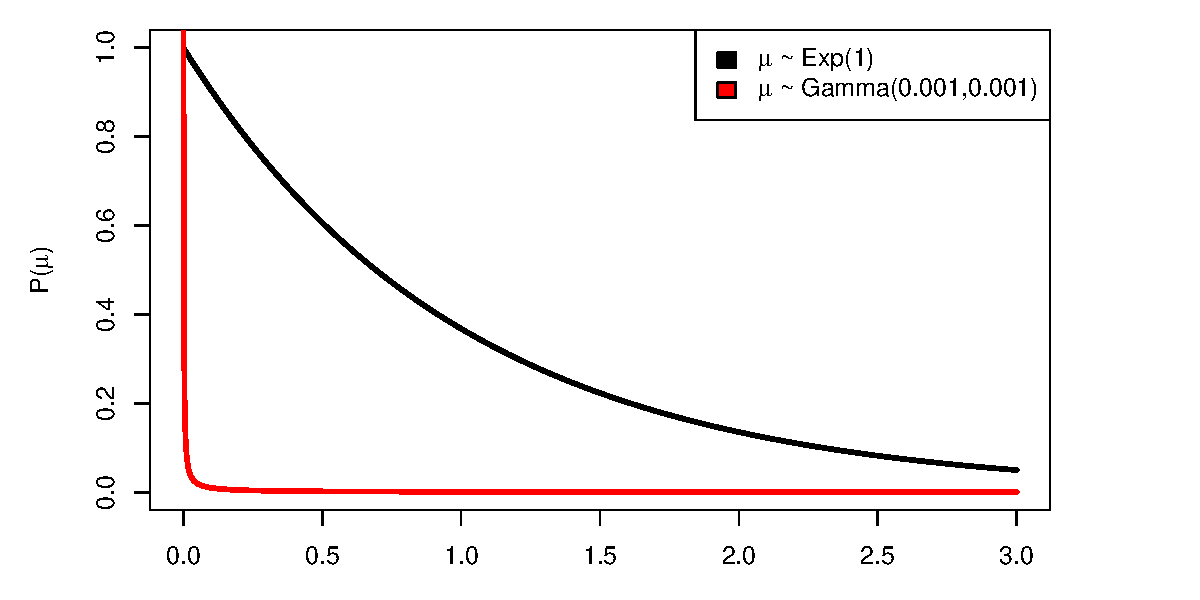
\includegraphics[width=0.7\linewidth,angle=0]{\ResourcePath figures/gamma.pdf}}
\label{fig:gamma_distribution}
\caption{Comparison of exponential distribution with $\alpha = 1$ and uninformative gamma distribution with parameters $\alpha=0.001$ and $\beta=0.001$.}
\end{figure}

The second and simplest way we can overcome the informativeness of the prior is to increase the amount of data we collect.
We can do that in our example by increasing the number of arrows we shoot.

\subsection{Exercise 4}

\begin{enumerate}[label=\textnormal{Step \arabic*)}]
	\item Increase the true mean arrow distance so that it is significantly larger than $\alpha$. How does this impact your estimate of $\mu$?
	\item Now use an uninformative Gamma$(0.001, 0.001)$ prior for $\mu$. Did your estimate of $\mu$ improve?
	\item Increase the number of arrows shot. How does this change the shape and scale of the posterior distribution?
\end{enumerate}

\bibliographystyle{sysbio}
\bibliography{\GlobalResourcePath refs}
